% !TEX program = lualatex
% =============================================================================
% Template LaTeX — Índice de Desconforto de Crédito (IDC)
%
% Compilar com: lualatex -interaction=nonstopmode template.tex (duas passagens)
%
% Uso para novo relatório mensal:
%   1. Copie esta pasta para outputs/report/update-YYYYMM/
%   2. Edite a seção "DADOS DO RELATÓRIO" abaixo
%   3. Preencha o corpo com o conteúdo real
%   4. Compile duas vezes
%   5. Gere o DOCX editável com python3 -m src.build_report_docx (veja PIPELINE.md)
% =============================================================================

\documentclass[11pt,a4paper]{article}

% --- Geometria (margens reproduzidas no DOCX gerado) ---------------------------
\usepackage[
  a4paper,
  left=30mm,
  right=30mm,
  top=25mm,
  bottom=25mm,
  headheight=14mm,
  headsep=6mm,
  footskip=10mm
]{geometry}

% --- Fonte e codificação (LuaLaTeX / XeLaTeX) ---------------------------------
\usepackage{fontspec}
\usepackage{microtype}

\setmainfont{TeX Gyre Pagella}   % clone de Palatino ≈ Cambria
\setsansfont{TeX Gyre Heros}     % clone de Helvetica ≈ Calibri
% Com MS Office instalado, descomente para fontes originais:
% \setmainfont{Cambria}
% \setsansfont{Calibri}[Scale=0.95]

% --- Português do Brasil ------------------------------------------------------
\usepackage[brazilian]{babel}
\usepackage{csquotes}

% --- Gráficos e tabelas -------------------------------------------------------
\usepackage{graphicx}
\graphicspath{{.}}
\usepackage{booktabs}
\usepackage{array}
\usepackage{caption}
\usepackage{subcaption}
\usepackage{float}

\captionsetup[figure]{
  format=plain, labelformat=simple, labelsep=period,
  labelfont={bf}, textfont=it, name=Figura, skip=0.4\baselineskip
}
\captionsetup[table]{
  format=plain, labelformat=simple, labelsep=period,
  labelfont={bf}, textfont=it, name=Tabela, skip=0.4\baselineskip,
  position=above
}

% Nota de fonte abaixo de figuras e tabelas.
% Para figuras, mantenha a fonte dentro do ambiente figure, imediatamente apos
% \caption{}. No anexo, [H] mantém gráfico, legenda e fonte como um bloco fixo,
% sempre em largura integral e com exatamente uma figura por página.
\newcommand{\fonte}[1]{%
  \par\vspace{0.2\baselineskip}%
  \small\textit{Fonte: #1}\par\vspace{0.8\baselineskip}%
}

% --- Tipografia e layout ------------------------------------------------------
\usepackage{xcolor}
\usepackage{setspace}
\usepackage{titlesec}
\usepackage[all]{nowidow}

\onehalfspacing

\titleformat{\section}{\Large\bfseries}{\thesection}{1em}{}
\titlespacing{\section}{0pt}{1.2\baselineskip}{0.6\baselineskip}
\titleformat{\subsection}{\large\bfseries}{\thesubsection}{1em}{}
\titlespacing{\subsection}{0pt}{1.0\baselineskip}{0.4\baselineskip}
\titleformat{\subsubsection}{\normalsize\bfseries}{\thesubsubsection}{1em}{}
\titlespacing{\subsubsection}{0pt}{0.8\baselineskip}{0.3\baselineskip}

% --- Cabeçalho e rodapé -------------------------------------------------------
\usepackage{fancyhdr}
\pagestyle{fancy}
\fancyhf{}
\fancyhead[L]{\small\itshape \reporttitle}
\fancyhead[R]{\small\itshape FGVcemif / FGV-EAESP}
\renewcommand{\headrulewidth}{0.4pt}
\renewcommand{\headrule}{\hbox to\headwidth{%
  \color{black!25}\leaders\hrule height 0.4pt\hfill}}
\fancyfoot[R]{\thepage}
\renewcommand{\footrulewidth}{0pt}

\fancypagestyle{firstpage}{
  \fancyhf{}
  \fancyfoot[R]{\thepage}
  \renewcommand{\headrulewidth}{0pt}
}

% --- Hiperlinks ---------------------------------------------------------------
\usepackage[unicode=true,colorlinks=true,
  linkcolor=black!70,urlcolor=black!70,citecolor=black!70]{hyperref}

% =============================================================================
%   DADOS DO RELATÓRIO — editar a cada atualização mensal
% =============================================================================

\newcommand{\reporttitle}{Índice de Desconforto de Crédito}

% Período de referência
\newcommand{\mesreferencia}{julho de 2026}
\newcommand{\mesref}{jul-2026}
\newcommand{\mesanterior}{jun-2026}
\newcommand{\competencia}{202609}
\newcommand{\mespublicacao}{setembro de 2026}
\newcommand{\proxdivulgacao}{outubro de 2026}
\newcommand{\mesproximo}{ago-2026}

% Datas fixas da série (raramente mudam)
\newcommand{\janelainicio}{jan-2014}   % início da janela exibida do IDC
\newcommand{\seriesinicio}{mar-2011}   % início das séries brutas C, I, Q

\newcommand{\reportsubtitle}{Nota Técnica de Atualização --- Divulgação \mespublicacao; competência \mesreferencia}
\newcommand{\reportdate}{Setembro de 2026}

% Autores
\newcommand{\authorone}{Lauro Gonzalez}
\newcommand{\authortwo}{Matheus L. Carrijo}
\newcommand{\authorthree}{Rafael Schiozer}

\hypersetup{
  pdftitle={\reporttitle},
  pdfauthor={\authorone; \authortwo; \authorthree},
  pdfsubject={Nota Técnica de Atualização do IDC},
  pdfkeywords={crédito, endividamento, Brasil, BCB, FGV}
}

% =============================================================================
\begin{document}
% =============================================================================

% --- Capa ---------------------------------------------------------------------
\hypersetup{pageanchor=false}
\begin{titlepage}
  \noindent\hfill
\includegraphics[width=79mm]{logo.png}

  \vspace{18mm}

  \begin{center}
    {\LARGE\bfseries \reporttitle\par}
    \vspace{3mm}
    {\large\itshape \reportsubtitle\par}
  \end{center}

  \vspace{12mm}

  \begin{flushright}
    \large
    \authorone\\[2pt]
    \authortwo\\[2pt]
    \authorthree
  \end{flushright}

  \vfill

  \begin{center}
    \reportdate
  \end{center}
\end{titlepage}
\hypersetup{pageanchor=true}
\thispagestyle{firstpage}

% =============================================================================
%   CONTEÚDO DO RELATÓRIO
% =============================================================================

\section{Resumo}

Com a publicação, em \mespublicacao, das Estatísticas Monetárias e de Crédito do
Banco Central do Brasil (competência \competencia), o Índice de Desconforto
de Crédito (IDC) foi recalculado e estendido até \mesreferencia{} --- último mês para
o qual há observação disponível da série de comprometimento de renda das famílias (SGS~29034),
que delimita o horizonte de cálculo do índice.

Em \textbf{\mesref}, o IDC foi de \textbf{0,963}, com alta de
\textbf{0,013~ponto} em relação aos \textbf{0,950} de
\textbf{\mesanterior}, ambos calculados com a safra \textbf{202609}.
O resultado foi o sétimo maior entre as \textbf{151} observações válidas
desde \textbf{jan-2014}. Na escala normalizada, em que \textbf{1,000}
representa o pior e \textbf{0,000} o melhor resultado histórico observado,
C e I marcaram \textbf{1,000}, enquanto Q ficou em \textbf{0,888}.

\section{Resultados de \mesreferencia}

\begin{table}[htbp]
  \centering
  \caption{Componentes brutos e valores normalizados do IDC --- \mesref.}
  \label{tab:componentes}
  \begin{tabular}{>{\raggedright\arraybackslash}p{8.0cm}rr}
    \toprule
    Indicador & Valor bruto & Valor normalizado \\
    \midrule
    IDC (média dos componentes normalizados)
      & ---
      & \textbf{0,963} \\
    C --- Comprometimento de renda das famílias com a dívida
      & 28,7\%
      & 1,000 \\
    I --- Inadimplência da carteira de crédito livre PF (90+ dias)
      & 7,8\%
      & 1,000 \\
    Q --- Participação do crédito oneroso no crédito livre PF
      & 24,4\%
      & 0,888 \\
    \bottomrule
  \end{tabular}
\end{table}

\fonte{Banco Central do Brasil (Estatísticas Monetárias e de Crédito,
divulgação \competencia), elaboração própria.}

Em relação à observação imediatamente anterior --- \textbf{\mesanterior}, quando o IDC
marcava \textbf{0,950} --- o índice subiu
\textbf{0,013~ponto} em \textbf{\mesref}.
O movimento concentrou-se em I: sua alta superou a redução de Q, enquanto C
permaneceu estável.

\begin{itemize}
  \item Comprometimento de renda (C) permaneceu em \textbf{28,7\%}
    (\textbf{0,0~p.p.}). O componente normalizado ficou em \textbf{1,000},
    correspondente ao pior posicionamento histórico observado. A estabilidade
    manteve o peso do serviço da dívida sobre a renda no máximo da amostra.

  \item Inadimplência (I) avançou de \textbf{7,4\%} para
    \textbf{7,8\%} (\textbf{+0,4~p.p.}), e seu valor normalizado passou de
    \textbf{0,943} para \textbf{1,000}. A taxa bruta atingiu o maior nível
    no horizonte calculável do IDC e respondeu pela alta mensal do índice.

  \item Participação do crédito oneroso (Q) caiu de \textbf{24,5\%} para
    \textbf{24,4\%} (\textbf{-0,1~p.p.}, com base nos valores não arredondados),
    e seu valor normalizado recuou de \textbf{0,907} para \textbf{0,888}.
    A menor participação das modalidades onerosas no crédito livre PF
    compensou parcialmente a piora de I.
\end{itemize}

Em conjunto, os dados indicam aumento do desconforto agregado em
\textbf{\mesref}, determinado pela inadimplência, com C ainda no máximo
histórico e alívio parcial em Q. O IDC permaneceu entre os níveis mais altos
da série, mas mede posição relativa no histórico, e não uma medida absoluta
de endividamento.

% SEÇÃO OPCIONAL — REVISÕES DOS DADOS
% Não inclua essa seção no relatório mensal por padrão.
% A auditoria de "python -m src.compare_releases YYYYMM" é sempre integral,
% mas uma revisão rotineira só recebe destaque público quando satisfaz a dupla
% materialidade: altera o IDC em pelo menos 0,010 ponto E afeta um elemento
% efetivamente discutido no relatório. Inversão de sinal, criação/remoção de
% recorde, invalidação de afirmação anterior, mudança metodológica relevante,
% mudança de fonte/cobertura ou correção de erro relevante podem justificar a
% seção independentemente do limiar. Reprocessamentos amplos
% da fonte só entram quando alteram materialmente a trajetória ou a interpretação.
% Quando necessária, insira aqui "Revisões dos dados" e mostre apenas as
% competências materiais ou indispensáveis para explicar a base de comparação,
% com três casas decimais. O registro técnico preserva todas as diferenças.

\section{Trajetória do índice}

A Figura~\ref{fig:indice} mostra que, após atingir \textbf{1,000} em
\textbf{fev-2026}, o IDC passou a \textbf{0,960} em \textbf{mar-2026},
\textbf{0,990} em \textbf{abr-2026}, \textbf{0,983} em \textbf{mai-2026},
\textbf{0,950} em \textbf{jun-2026} e \textbf{0,963} em
\textbf{jul-2026}. A Figura~\ref{fig:componentes} evidencia que a alta mais
recente refletiu o avanço de I para seu máximo no horizonte calculável do
IDC; C permaneceu no máximo da amostra, enquanto Q recuou.
\section{Próxima atualização}

A próxima atualização é esperada para \proxdivulgacao; o IDC será estendido para
\mesproximo{} caso a série de comprometimento de renda (SGS~29034) avance até lá.

\section*{Notas}

\begingroup\footnotesize

Sobre o IDC. O Índice de Desconforto de Crédito (IDC) é construído a partir de
três séries do Sistema Gerenciador de Séries Temporais (SGS) do Banco Central do Brasil:
comprometimento de renda das famílias com o serviço da dívida (SGS~29034), inadimplência
da carteira de crédito livre PF --- atrasos superiores a 90 dias (SGS~21112) --- e
participação do crédito oneroso, definida como a parcela do saldo total de crédito
livre para pessoa física (SGS~20570) nas modalidades cheque especial (SGS~20573), crédito
pessoal não consignado (SGS~20574), cartão de crédito rotativo (SGS~20587) e cartão de
crédito parcelado (SGS~20588). Cada componente é
normalizado pelo método min-max com janela expansiva, a partir de \seriesinicio; o índice
é exibido a partir de \janelainicio, após o período de aquecimento da janela, e corresponde
à média simples dos três componentes normalizados, contido no intervalo [0,~1]. Por
construção, o IDC mede a posição relativa do mês corrente em relação ao histórico observado
pelo índice. O relatório de divulgação está disponível em
\url{https://eaesp.fgv.br/producao-intelectual/indice-desconforto-credito-idc}.

Revisões dos dados. Os valores históricos do IDC são recalculados a cada edição
com a safra mais recente dos dados do Banco Central. Revisões com efeito material
sobre o índice ou sua interpretação são descritas no relatório; a série
disponibilizada incorpora todas as revisões identificadas.

Citação recomendada. Gonzalez, L.; Carrijo, M.~L.; Schiozer, R.
\textit{Índice de Desconforto de Crédito (IDC).} FGVcemif/FGV-EAESP\@.
\endgroup

% As figuras ficam em um anexo próprio, uma por página. Assim, nenhuma figura
% disputa espaço com o corpo textual ou precisa ser reduzida para caber.
\clearpage
\section*{Anexo de figuras}

\begin{figure}[H]
  \centering
  \IfFileExists{index.png}{%
    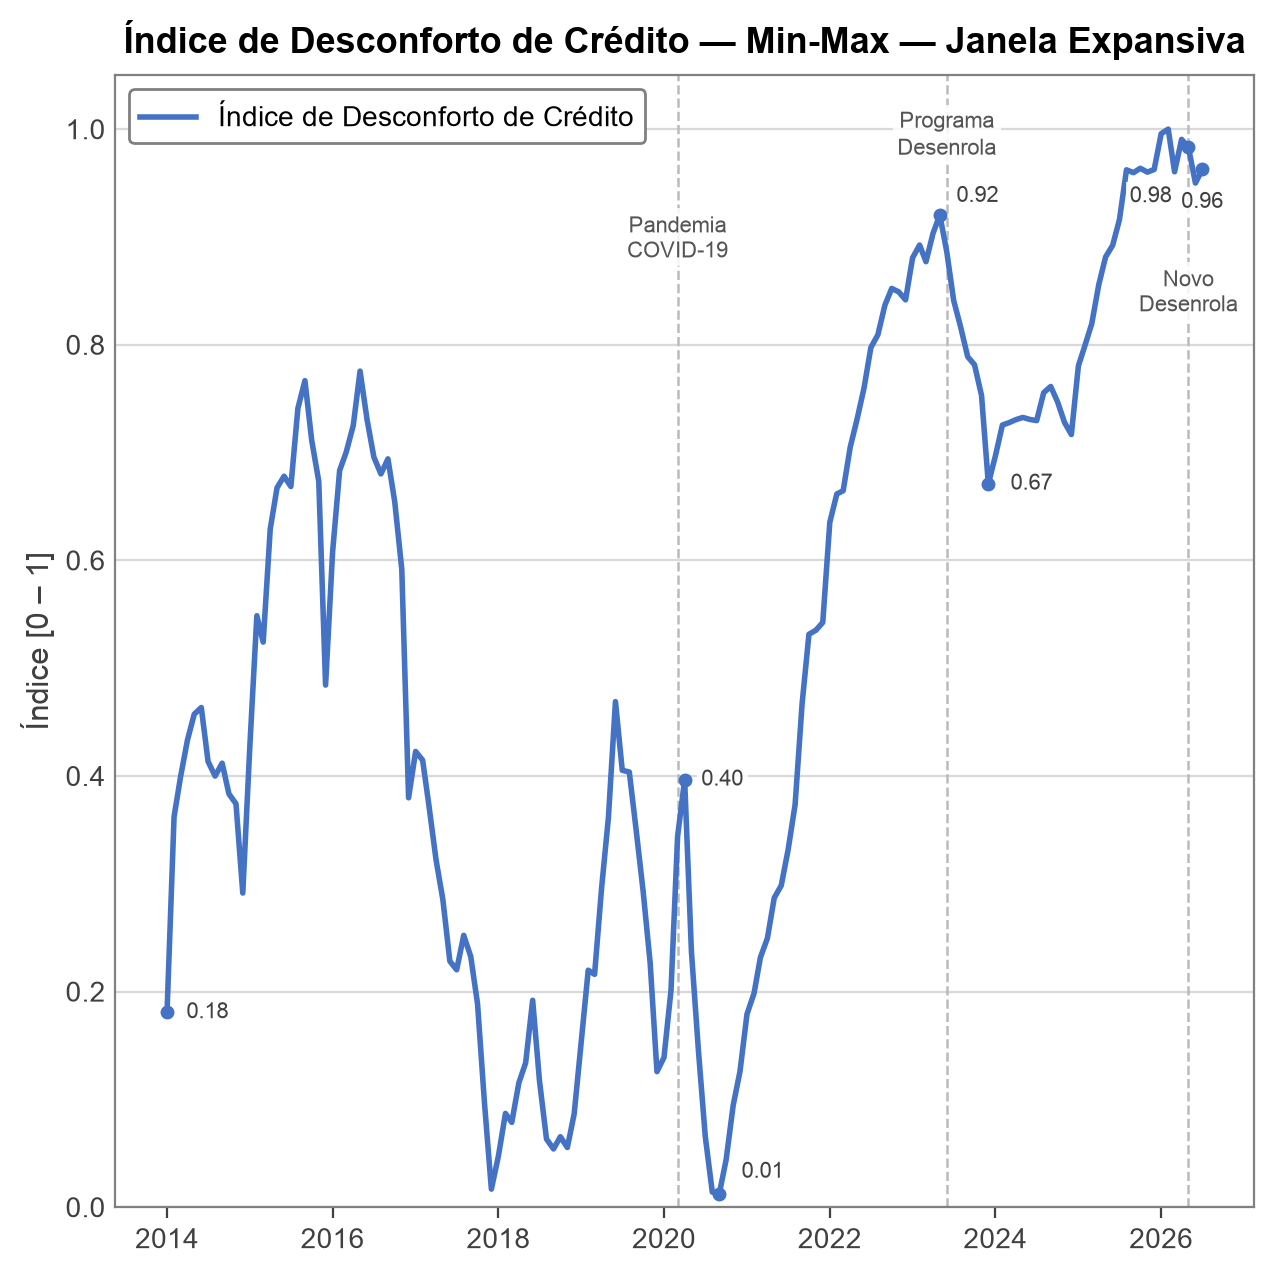
\includegraphics[width=\linewidth]{index.png}%
  }{%
    \fbox{\rule{0pt}{14cm}%
      \rule{\dimexpr\linewidth-2\fboxsep-2\fboxrule\relax}{0pt}}%
  }
  \caption{Evolução do Índice de Desconforto de Crédito (\janelainicio{} a \mesref).}
  \label{fig:indice}
  \fonte{BCB, elaboração própria.}
\end{figure}

\clearpage
\begin{figure}[H]
  \centering
  \IfFileExists{components_raw.png}{%
    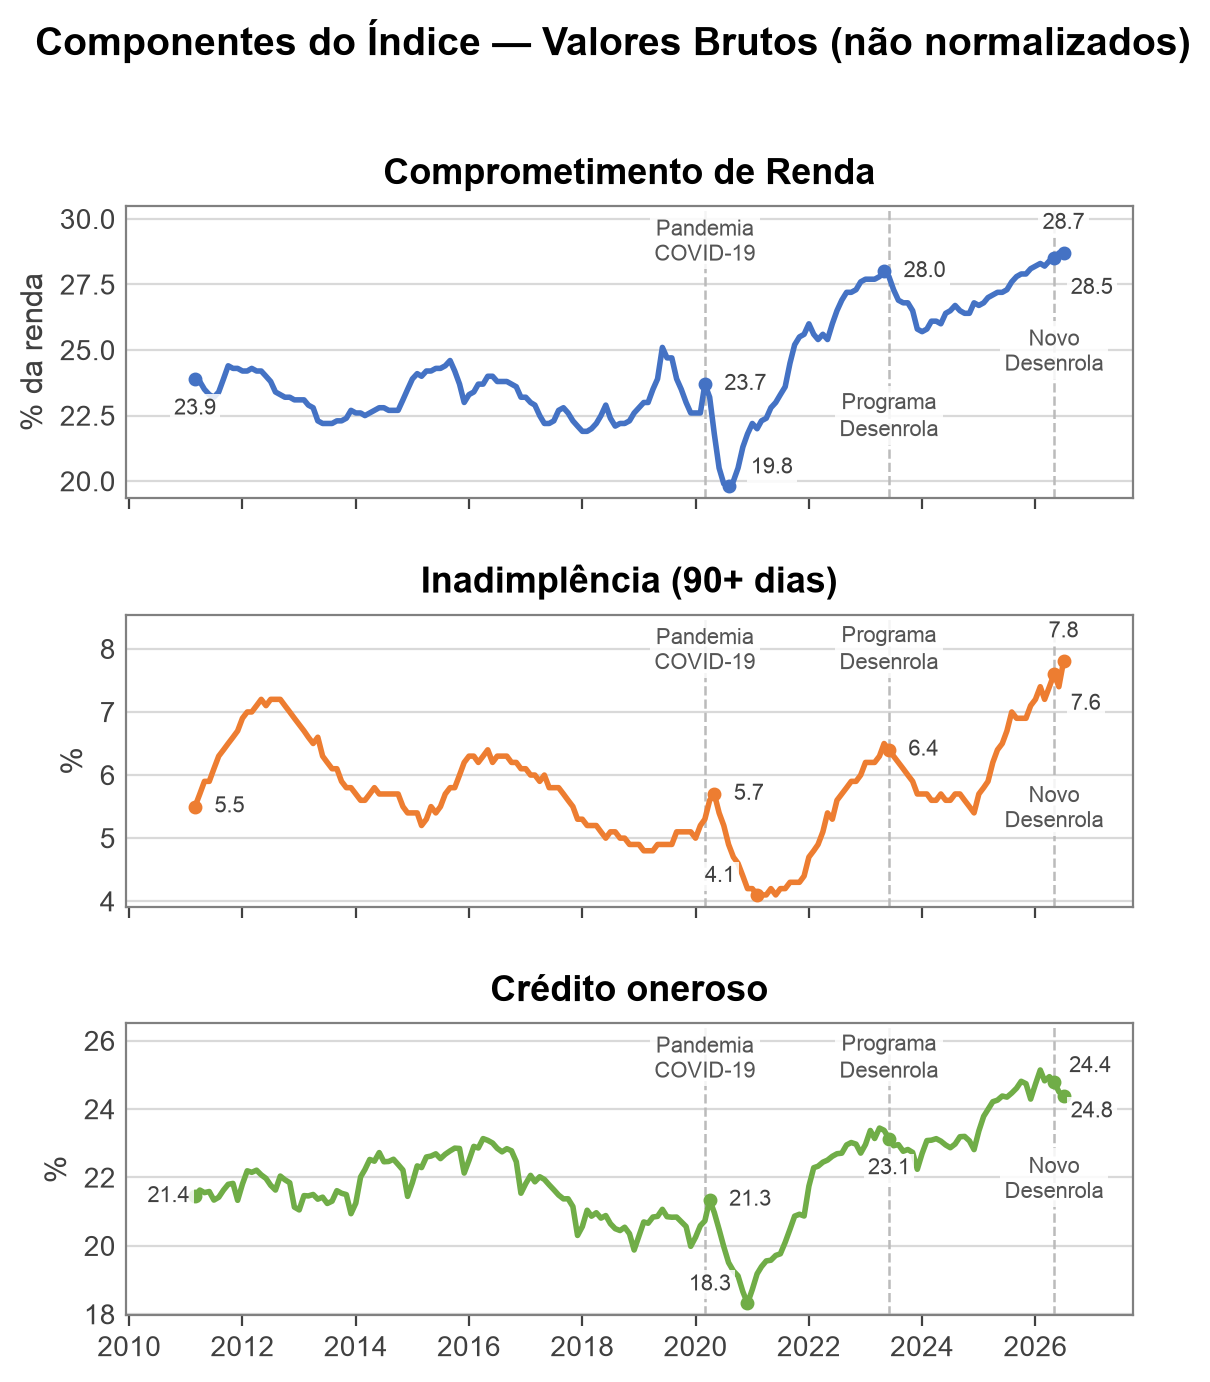
\includegraphics[width=\linewidth]{components_raw.png}%
  }{%
    \fbox{\rule{0pt}{17cm}%
      \rule{\dimexpr\linewidth-2\fboxsep-2\fboxrule\relax}{0pt}}%
  }
  \caption{Evolução das componentes brutas C, I e Q (\seriesinicio{} a \mesref).}
  \label{fig:componentes}
  \fonte{BCB, elaboração própria.}
\end{figure}

\end{document}
